\section{Uncertainty and Sensitivity Analysis}\label{sec:uq}
Uncertainty enters through the parameters, the usage and the model structure. Unless stated, RP-63 is new and starts
full at 25\,$^\circ$C; intervals are 90\,\% parameter intervals, median [5\,\%, 95\,\%].

\subsection{Parameter uncertainty}
\begin{figure}[t]
  \centering
  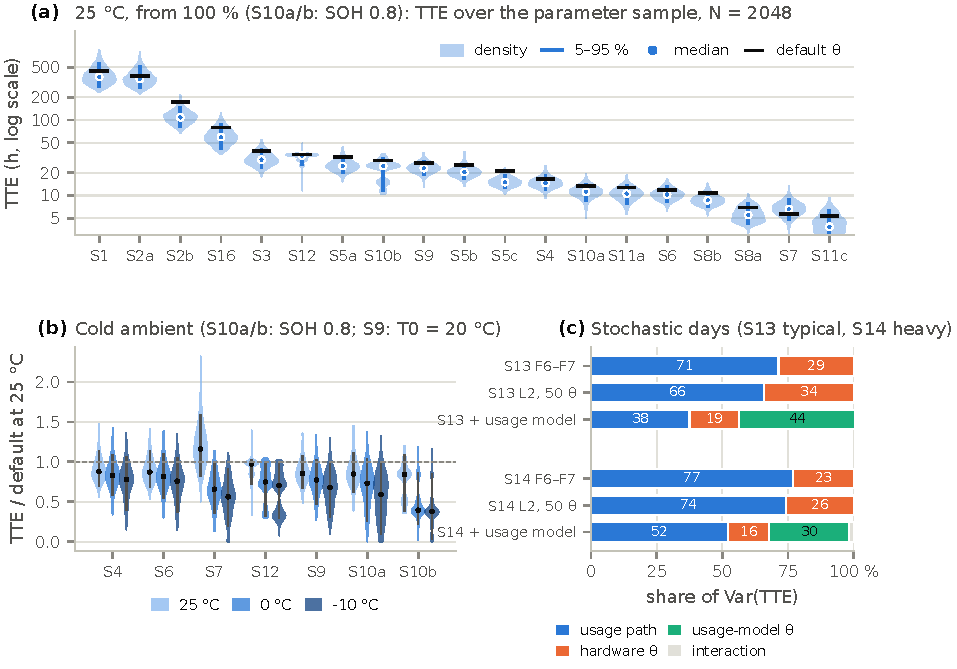
\includegraphics[width=0.86\textwidth]{figures/fig_uq_violins.pdf}
  \caption{Parameter uncertainty ($N=2048$). (a) TTE at 25\,$^\circ$C (log scale; the hike S9 also at
  25\,$^\circ$C); the nominal prediction (black bar, ``default $\theta$'') lies above the median except for gaming
  (S7). (b) Cold widens the distributions downwards, most for the aged pack (S10a/b). (c) Share of Var(TTE) on
  random days: usage randomness outweighs hardware.}
  \label{fig:uq_violins}
\end{figure}
One joint scrambled Sobol' sample of all prior ranges in \cref{tab:params} is run through L2 for every scenario
(\cref{fig:uq_violins}; 25\,$^\circ$C intervals in \cref{tab:baseline}). \textbf{The defaults are optimistic:} the medians are
3--38\,\% shorter than the nominal values, e.g.\ social feed (S4) 14.6 [11.7, 18.8]\,h against 16.6\,h and scheduled
day (S12) 33.9 [25.2, 35.4]\,h against 34.9\,h. The cause is energy (L0 gives the same ratios;
\cref{sec:params}). Gaming is the exception
(6.6 [4.7, 9.0]\,h against 5.7\,h), because draws with a low skin limit throttle harder and run longer (F5). At
25\,$^\circ$C the energy shares of F1 predict the spread: the rule $\mathrm{CV}_{\TTE}^2\approx\mathrm{CV}_{E_u}^2+
\sum_i\phi_i^2\mathrm{CV}_{P_i}^2$ (energy shares $\phi_i$) matches the simulated CV within a ratio of 0.87--1.32
in 90\,\% of the cases (median 1.09).

\textbf{Cold widens the uncertainty, and L0 fails there.} At $-10\,^\circ$C the social-feed median moves only to
13.0\,h, but the 5\,\% quantile falls from 11.7 to 6.7\,h: brown-out ends 95\,\% of the runs, with median stranded charge
9.5\,\% (95\,\% quantile 54\,\%). On an aged pack (SOH 0.8) the interval is 7.8 [1.3, 12.8]\,h against a nominal
12.1\,h. The CV rule now underestimates the spread by factors of 1.3--2.1 for constant screen-on loads on a new
pack (3.0 for the scheduled day) and 3.4--6.6 on the aged pack, because the voltage limit carries the uncertainty. The chance that the scheduled day dies before 23:00 rises from 0.002 at
25\,$^\circ$C to 0.37 at $-10\,^\circ$C (0.92 for the aged pack).

\subsection{Random usage}
For the random days of \cref{sec:usage}, 2000 L2 paths give $39.6\pm7.1$\,h (mean $\pm$ SD; 5, 50 and 95\,\%
quantiles 27.8, 39.7 and 50.9\,h) for the typical and $21.5\pm4.9$\,h (13.5, 21.5, 29.7\,h) for the heavy profile. With identical
hardware a lucky typical day lasts almost twice as long as an unlucky one (\cref{fig:ctmc}), and a heavy user's
phone fails to last 24\,h with probability 0.70 (typical 0.015). \textbf{Usage randomness outweighs hardware:} in
full L2 (50 draws $\times$ 200 paths) the paths carry 66\,\% (95\,\% CI 55--78) of Var(TTE) on the typical and
74\,\% (65--83) on the heavy day (F6--F7 over all 2048 draws: 71 and 77\,\%; \cref{fig:uq_violins}c). With
uncertain usage-model rates the typical split is 38\,\% path, 19\,\% hardware and 44\,\% usage model: who the user
is matters as much as what they do on a given day. F6 needs a per-draw voltage correction: a pre-registered check
with one pooled L2/L0 factor fails, because the L2/L0 ratio varies across draws (0.74--0.98) with the voltage
layer, not with the usage model. Stretching all sessions by $\kappa$ confirms F7's $\mathrm{SD}\propto\sqrt\kappa$
within about 2\,\% for $\kappa\le1$ (F7 is 10\,\% high at $\kappa=4$). Heavy-tailed (lognormal, CV 1.5) sessions
leave the mean nearly unchanged ($+1.6\,\%$) but widen the SD by 10--16\,\%.

\begin{figure}[t]
  \centering
  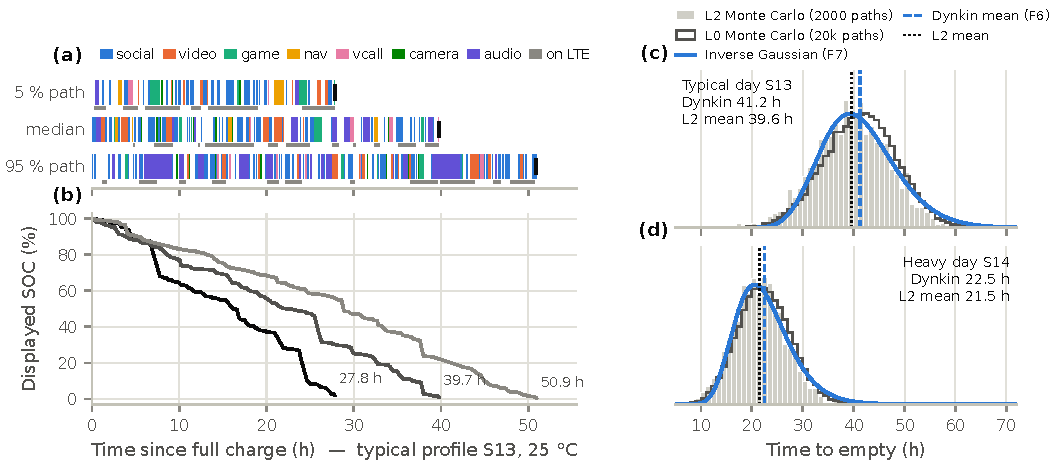
\includegraphics[width=0.87\textwidth]{figures/fig_ctmc_tte.pdf}
  \caption{Random days. (a) Activities of the typical-day paths at the 5\,\%, 50\,\% and 95\,\% TTE quantiles (grey
  bars: on LTE) and (b) their displayed SOC under L2. (c, d) TTE histograms of 2000 L2 and 20\,000 L0 paths with
  the F6 (Dynkin) mean and the inverse-Gaussian law of F7.}
  \label{fig:ctmc}
\end{figure}

\subsection{Parameter sensitivity: three regimes}
Local elasticities ($\pm5\,\%$), one-at-a-time (OAT) sweeps over the prior ranges and Sobol' indices of 24 factor
groups (Saltelli and Jansen estimators \cite{SALT10,JANS99,SALIB17}) agree on three regimes. Constant loads use the F2/F4/F5 surrogate (within 0.77\,\% of L2); gaming, the cold
cases and the weak-signal call (surrogate error 6.9\,\% near thermal shutdown) use full L2.

\begin{figure}[t]
  \centering
  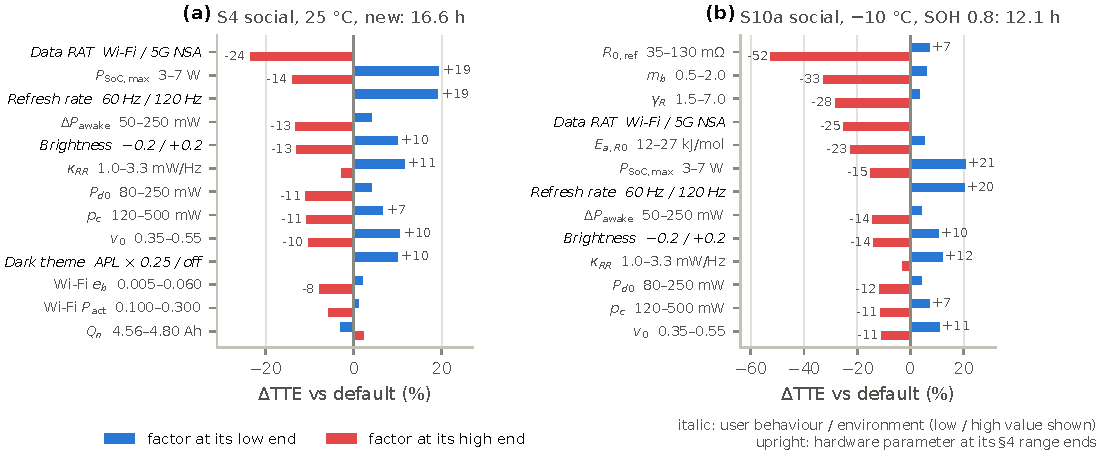
\includegraphics[width=0.86\textwidth]{figures/fig_tornado.pdf}
  \caption{One-at-a-time sweeps over the prior ranges: change of TTE against the nominal (``default'') value with
  each factor at its low (blue) or high (red) end. (a) Energy-limited social feed at 25\,$^\circ$C: user choices
  (italic) rival the widest hardware ranges. (b) Voltage-limited aged pack at $-10\,^\circ$C: pack resistance and burst
  size lead.}
  \label{fig:tornado}
\end{figure}

\paragraph{Energy-limited (25\,$^\circ$C).} Capacity has elasticity $+1.00$ and the processor voltage offset $v_0$
has $-0.46$, but the pack resistance only $-0.007$. The first-order indices sum to $\ge0.95$, every cell or thermal
group has $S_{Ti}\le0.02$, and the active component carries the variance: display in reading (0.68), processor in
the social feed (0.50), the 5G radio in 5G video (0.54). User choices span as much as the widest hardware range
(\cref{fig:tornado}a; social feed, $P_{\mathrm{SoC,max}}$: $+19\,\%$/${-14}\,\%$): 5G instead of Wi-Fi costs
24\,\% and a 60\,Hz cap gains 19\,\%.

\paragraph{Voltage-limited (cold and aged).} At $-10\,^\circ$C and SOH 0.8 the ranking inverts
(\cref{fig:tornado}b): pack resistance (OAT
$-52\,\%$ at the top of its range, $S_{Ti}=0.47$) and burst size ($-33\,\%$, 0.25) lead, and the TTE CV rises to
0.47--0.56 (0.13--0.21 at 25\,$^\circ$C with good signal).

\paragraph{Thermal-limited (gaming).} Enclosure (0.40), skin resistance (0.38) and throttle settings (0.18) dominate; each kelvin of extra skin limit costs 4.5\,\% of gaming time, and a
35\,$^\circ$C room gains 81\,\% (F5). Interactions are small: $1-\sum_iS_i\le0.07$, and its 95\,\% interval
contains zero in every scenario.

\subsection{Structural sensitivity}\label{sec:structural}
\begin{table}[t]\centering\footnotesize
\caption{Structural variants: change of TTE (\%) and of stranded charge (points) against L2. S4 social, S7 gaming,
S12 scheduled day, S13 typical random day, S9 cold hike, S10a social. Not shown: X11 brightness law, X12
energy-fraction display, X13 processor leakage, X14 audio on a low-power signal processor (S16 $+63\,\%$), X17
$t^{0.75}$ calendar law, X18 other OCV stretches.}
\label{tab:structural}
% T4: structural variants, Delta TTE (%) and Delta s_off (percentage points) against the full model, same solver and step.
% Compact version for the paper. Not shown (text or caption only): X5n (2RC with equal total R1: 0.0 everywhere),
% X11a/b (brightness law), X12 (SOC output D2), X13 (processor leakage), X14 (audio on DSP: S13 +2.7, S16 +63.1),
% X17 (calendar law t^0.75), X18a/b (OCV stretch).
\setlength{\tabcolsep}{4pt}%
\begin{tabular}{@{}llrrrrrrrr@{}}
\toprule
 & & \multicolumn{4}{c}{25\,$^\circ$C, new: $\Delta$TTE (\%)} & \multicolumn{4}{c}{$-20\,^\circ$C, SOH 0.8} \\
\cmidrule(lr){3-6}\cmidrule(l){7-10}
 & & & & & & \multicolumn{2}{c}{S9 hike} & \multicolumn{2}{c}{S10a social} \\
\cmidrule(lr){7-8}\cmidrule(l){9-10}
ID & Variant & S4 & S7 & S12 & S13 & $\Delta$TTE & $\Delta s_\mathrm{off}$ & $\Delta$TTE & $\Delta s_\mathrm{off}$ \\
\midrule
X1 & L0 energy bucket & +0.9 & +0.5 & +0.3 & +3.9 & +79.0 & $-$44.2 & +31.3 & $-$23.3 \\
X2 & L1, isothermal & 0.0 & $-$22.7 & $-$1.0 & $-$5.0 & $-$36.5 & +21.1 & +23.8 & $-$20.3 \\
X3 & L2 isothermal, no throttling & 0.0 & $-$22.9 & $-$1.0 & $-$5.1 & $-$10.8 & +6.2 & $-$11.5 & +9.1 \\
X4 & constant current, $I=P/3.87$\,V & +0.1 & +0.1 & 0.0 & +0.2 & +16.2 & $-$9.4 & +11.4 & $-$8.5 \\
X5 & two RC branches & 0.0 & 0.0 & 0.0 & 0.0 & +2.7 & $-$1.5 & +1.4 & $-$1.0 \\
X6 & $R_0$ split: protection circuit + cell & 0.0 & $-$0.3 & 0.0 & $-$0.1 & +52.7 & $-$30.6 & +22.9 & $-$18.1 \\
X7 & no sub-second burst envelope & 0.0 & 0.0 & 0.0 & 0.0 & 0.0 & 0.0 & +24.9 & $-$20.8 \\
X8 & single threshold, $V_\mathrm{sys}=V_\mathrm{cut}$ & $-$1.1 & $-$1.7 & $-$0.2 & $-$1.1 & 0.0 & 0.0 & $-$20.9 & +17.0 \\
X9 & kinetic battery (KiBaM) instead of RC & $-$0.2 & $-$0.3 & $-$0.1 & $-$0.2 & $-$29.8 & +17.2 & $-$1.6 & +0.9 \\
X10 & radio tail as an ODE state & 0.0 & 0.0 & 0.0 & $-$0.4 & $-$1.3 & +0.6 & 0.0 & 0.0 \\
X15 & lognormal sessions, CV 1.5 & -- & -- & -- & +1.6 & -- & -- & -- & -- \\
X16 & diurnal usage chain & -- & -- & -- & +8.1 & -- & -- & -- & -- \\
\bottomrule
\end{tabular}

\end{table}
Each variant replaces one assumption (\cref{tab:structural}). \textbf{At 25\,$^\circ$C the circuit form hardly
matters:} constant current, two RC branches, a split $R_0$, KiBaM or another OCV stretch change TTE by
under 1\,\%, and L0 is at most 1.9\,\% long on constant loads (3.9--4.7\,\% on random days). Throttling is indispensable for gaming ($-23\,\%$ without
it, $-57\,\%$ at 35\,$^\circ$C), and the load laws matter more (audio on a low-power signal processor, X14:
$+63\,\%$ for screen-off music).
\textbf{Cold and aged, the form dominates:} L0 overstates the hike by 79\,\% and misses 44 points of stranded charge,
the split $R_0$ adds 53\,\%, KiBaM removes 30\,\%, and dropping the burst envelope or merging the two thresholds
moves the aged social feed by $+25$ or $-21\,\%$. Without self-heating the aged scheduled day at 0\,$^\circ$C is
53\,\% shorter. A $t^{0.75}$ calendar law (X17) reaches SOH 0.8 after 2.66 instead of 2.86 years.

\subsection{Usage fluctuations}
Alternating 0.4 and 2.0\,W instead of a constant 1.2\,W costs about 0.5\,\% at 25\,$^\circ$C for periods of 10\,s to
1\,h. On an aged pack at $-10\,^\circ$C with 3\,W sub-second bursts it costs 7.3--8.4\,\% (periods up to 10\,min),
because the high phases trigger the brown-out earlier (stranded charge 9.2\,\% at constant load, 15.6--16.6\,\%
alternating). \textbf{Order matters most
in the cold.} Reversing the scheduled day lengthens it by 5.4\,\% at 25\,$^\circ$C, as in L0 (pure scheduling), but
by 96\,\% (12.0 to 23.5\,h) on the aged pack at $-10\,^\circ$C: in the forward order the 18:00 game browns the phone
out at 32\,\% charge. L0 gives $+26\,\%$, so 70 points come from the voltage limit. Per-session jitter of $\pm30\,\%$
in brightness, picture level and traffic changes the SD by under 0.3\,\%.

\begin{keybox}[Key finding]
Defaults are optimistic, and usage randomness outweighs hardware uncertainty. At 25\,$^\circ$C TTE is an energy
budget that any circuit form reproduces within 1\,\%; cold and aged, pack resistance, burst size and \emph{when}
heavy use happens decide the day.
\end{keybox}
